\documentclass[12pt]{article}
\usepackage{epsfig}
\usepackage{tabu}

\textheight     9.0truein
\textwidth      6.5truein
\topmargin     -0.5truein
\oddsidemargin  +0.0truein
\evensidemargin +0.0truein

\newtheorem{theorem}{Theorem}[section]
\newtheorem{claim}[theorem]{Claim}
\newtheorem{lemma}[theorem]{Lemma}
\newtheorem{proposition}[theorem]{Proposition}
\newtheorem{corollary}[theorem]{Corollary}

\newenvironment{proof}[1][Proof]{\begin{trivlist}
\item[\hskip \labelsep {\bfseries #1}]}{\end{trivlist}}
\newenvironment{definition}[1][Definition]{\begin{trivlist}
\item[\hskip \labelsep {\bfseries #1}]}{\end{trivlist}}
\newenvironment{example}[1][Example]{\begin{trivlist}
\item[\hskip \labelsep {\bfseries #1}]}{\end{trivlist}}
\newenvironment{remark}[1][Remark]{\begin{trivlist}
\item[\hskip \labelsep {\bfseries #1}]}{\end{trivlist}}

\newcommand{\qed}{\nobreak \ifvmode \relax \else
      \ifdim\lastskip<1.5em \hskip-\lastskip
      \hskip1.5em plus0em minus0.5em \fi \nobreak
      \vrule height0.75em width0.5em depth0.25em\fi}

\title{Contracted 1-Tunnel within the Macro-Motion Union}
\author{}
\begin{document}
\maketitle


\begin{theorem} A Robot $R$ consisting of two 2x2 contracted Modules $M_a$, $M_b$ cannot perform a 1-Tunnel move within the union of the macro-motion, i.e. occupy no space outside other than the spaces occupied at the beginning or end of the macro-motion. Assuming that units cannot switch which module they belong to, but can switch their ordering within the module.
\\\\
To simplify this proof, we label each unit block space as below. $w.l.o.g$ we assume module $M_a$ is above module $M_b$ at the start, and the move terminates with module $M_a$ to the left of module $M_b$.


\begin{figure}[h!]
\centering
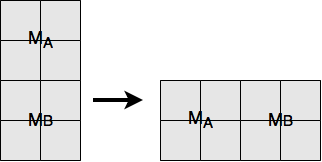
\includegraphics[scale=0.4]{ModuleLocations.png}
\caption{Start and end configurations of contracted 1-tunnel macro-motion.}
\label{fig:ModuleLocations}
\end{figure}

\begin{figure}[h!]
\centering
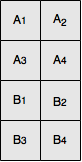
\includegraphics[scale=0.4]{UnitLabels.png}
\caption{Contracted 1-tunnel starting configuration with labeled units. Notice that in the figure below, unit $A_1$ starts in space 1, and $B_1$ starts in space 4.}
\label{fig:UnitLabels}
\end{figure}

\begin{figure}[h!]
\centering
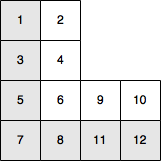
\includegraphics[scale=0.4]{InsideOutside.png}
\caption{Union of the contracted 1-tunnel macro-motion with grey $OUTSIDE$ spaces and white $INSIDE$ spaces labeled by number.}
\label{fig:InsideOutside}
\end{figure}

\begin{definition} An $INSIDE$ unit space is a unit space belonging to the set $\{2,4,6,9,10\}$.
\end{definition}
\begin{definition} An $OUTSIDE$ unit space is a unit space belonging to the set $\{1,3,5,7,8,11,12\}$.
\end{definition}

\begin{lemma} A macro-motion of this type requires moving a unit in an $INSIDE$ unit space to an $OUTSIDE$ unit space or vis-versa.
  \begin{proof} 
    Before the macro-motion, $M_a$ has two units $a_1, a_2 \in OUTSIDE$, 
    and two units, $a_3, a_4 \in INSIDE$. After the macro-motion, since 
    module $M_a$ occupys the space that $M_b$ occupied at the 
    beginning of the macro-motion, it has 1 unit inside and 3 units 
    outside. Therefore, one unit from module $M_a$ must have moved 
    from $INSIDE$ to $OUTSIDE$ during the macro-motion. 
  \end{proof}
\end{lemma}
It follows that to stay in the union of the macro-motion, all units must be either $INSIDE$ or $OUTSIDE$. i.e. $UNITS = INSIDE \cup OUTSIDE$, and $INSIDE \cap OUTSIDE = \emptyset$

\begin{definition} Let a $Transfer(s_{in}, s_{out})$ signify the movement of a unit from an $INSIDE$ space to an $OUTSIDE$ space or vis-versa. Note that this is only a \textbf{valid} transfer if exactly one of the two spaces is empty. It follows that all transfers are invertible. 
\end{definition}

\begin{lemma} If it is possible to transfer an $INSIDE$ unit, then it is possible to transfer an $OUTSIDE$ unit using inverse movements.
\end{lemma}
\begin{proof}
Since all movements are invertible, it is possible to transform the end state of the $IN \rightarrow OUT$ movement to the begin state of the $IN \rightarrow OUT$ movement. This new inverted movement will transform the same unit from $OUT \rightarrow IN$.
\end{proof}
\begin{lemma} All valid transfers involve a transfer to or from space 6
\end{lemma}
\begin{proof}
We will start by listing all possible transfers from $IN$ to $OUT$ and vis-versa.
\begin{enumerate}
\item $1 \leftrightarrow 2$
\item $3 \leftrightarrow 4$
\item $5 \leftrightarrow 6$
\item $6 \leftrightarrow 8$
\item $9 \leftrightarrow 11$
\item $10 \leftrightarrow 12$
\end{enumerate}
Transfers 1,2 are only possible given a concurrent transfer 3, as the upper blocks have no room to perform a horizontal extention or contraction and must rely on connections to units below to move them in space. Similarly transfers 5,6 are only possible given a concurrent transfer of case 4. Therefore all transfers require either case 3 or 4, which both involve space 6.
\end{proof}
\begin{claim} Given the constraints in stated in theorem 0.1 (reference appendix). It is impossible to perform a transfer given the initial configuration of units in the one-tunnel macro-motion.

By Contradiction. Assume not, i.e. There exists a basic movement that will move a block from an $INSIDE$ space to an $OUTSIDE$ space or vis-versa with a start state with 3 inside blocks and 5 outside blocks. By lemma 0.4 we only need to consider transfers that involve unit 6. 
\begin{itemize}
\item Case 1: Transfer(5,6) via arm connected to space 9
\item Case 2: Transfer(5,6) via arm connected to space 11
\item Case 3: Transfer(6,8) via arm connected to space 4
\item Case 4: Transfer(6,8) via arm connected to space 3
\end{itemize}
Case 3 is a vertical version of case 1. Case 4 a vertical version of case 2. Therefore we will only consider cases 1 and 2. Since all movements are invertible ***lemma, w.l.o.g. we only need to consider the transfers in cases 1,2 that involve arm extensions, i.e. move units from $IN$ to $OUT$.

\begin{lemma}
In cases 1,2 $IN \rightarrow OUT$, spaces 1,3,5 must be empty.
\end{lemma}
\begin{proof}
\begin{itemize}
\item Case 1: *** Picture Transfer(5,6) $IN \rightarrow OUT$ connected to space 9. For this transfer to be valid spaces 1, 3, 5, must be empty. Space 5 must be empty because when $arm(6,9)$ extends a unit in 5 would go outside the union. Space 3 must be empty because if space 3 is filled then it must be connected to the rest of the robot with $arm(3,4)$. Space 4 must be connected with $arm(4,6)$. These arms would make it so that when $arm(6,9)$ extends the unit in space 3 will go outside the union. Space 1 must be empty for a similar reason as space 3.
\item Case 2: *** Picture Transfer(5,6) $IN \rightarrow OUT$ connected to space 11. For this transfer spaces 1,3,5,7 must be empty. Spaces 1,3,5 must be empty for the reasons listed in case 1 as unit 6 is still transfering to space 5. Unit 7 must be empty as unit 8 will occupy that space in the end state. 
\end{itemize}
\end{proof}
By the pidgen hole principle, it is impossible for both spaces 1,3,5 to be empty and the robot to have 5 outside units and 3 inside units. Therefore all transfers are impossible from the initial robot state. 
\end{claim}
Since a transfer is required for a contracted 1-tunnel macro-motion, and no transfers are possible within the union from the start state, then the contracted 1-tunnel move is not possible given the constraints as above. 
\end{theorem}

\section{Appendix}
Theorem 0.1 constraints:
\begin{enumerate}
\item Modules are 2x2
\item Robot is contracted
\item Units must remain in module that they are initially assigned, but not in the same configuration within that module.
\item Robot must remain connected throughout the macro-motion
\item All units in Modules $M_a$ and $M_b$ must stay within the union of the macro-motion.
\end{enumerate}

\end{document}